\section{Overall System Architecture}
The overall architecture of the proposed Indian Sign Language recognition system is designed to process visual gesture input and convert it into meaningful textual and audio output. The system operates through a multi-stage deep learning pipeline that extracts both spatial and temporal information from the video sequence.

The complete workflow of the proposed system is illustrated in Fig.~\ref{fig:arch-proposed}, which presents the architecture diagram of the model and the interaction between different processing modules. As shown in Fig.~\ref{fig:arch-proposed}, the system begins with the acquisition of video input captured using a standard RGB camera. The input video is decomposed into individual frames through preprocessing. These frames are resized and normalized to maintain consistent spatial dimensions and improve numerical stability during model training and inference.

The processed frames are passed to the feature extraction stage where the system learns important visual characteristics of the gesture. Two complementary streams are used to capture different aspects of sign language gestures. The first stream performs spatial feature extraction using EfficientNet \cite{yenisari2025deep}, which learns visual patterns such as hand shape, finger positioning, and gesture orientation. In parallel, the second stream performs temporal feature extraction using a CNN--RNN framework that analyzes frame sequences to capture motion dynamics and gesture transitions over time.

After feature extraction, the system applies a multi-feature attention mechanism. This module assigns adaptive weights so the model focuses on informative frames and suppresses less relevant information. The weighted spatial and temporal features are combined using a feature fusion module to create a unified spatiotemporal representation.

The fused feature sequence is then processed by a sequence modeling component that captures contextual relationships between frames. A Connectionist Temporal Classification (CTC) layer aligns predicted labels with input sequences without requiring precise frame-level annotations. Finally, the recognized gesture sequence is converted into readable text and optionally transformed into speech output using a text-to-speech module.

Thus, the architecture integrates multiple deep learning components to effectively capture gesture appearance, motion dynamics, and contextual relationships, enabling accurate real-time recognition of Indian Sign Language gestures.

\begin{figure}[H]
\centering
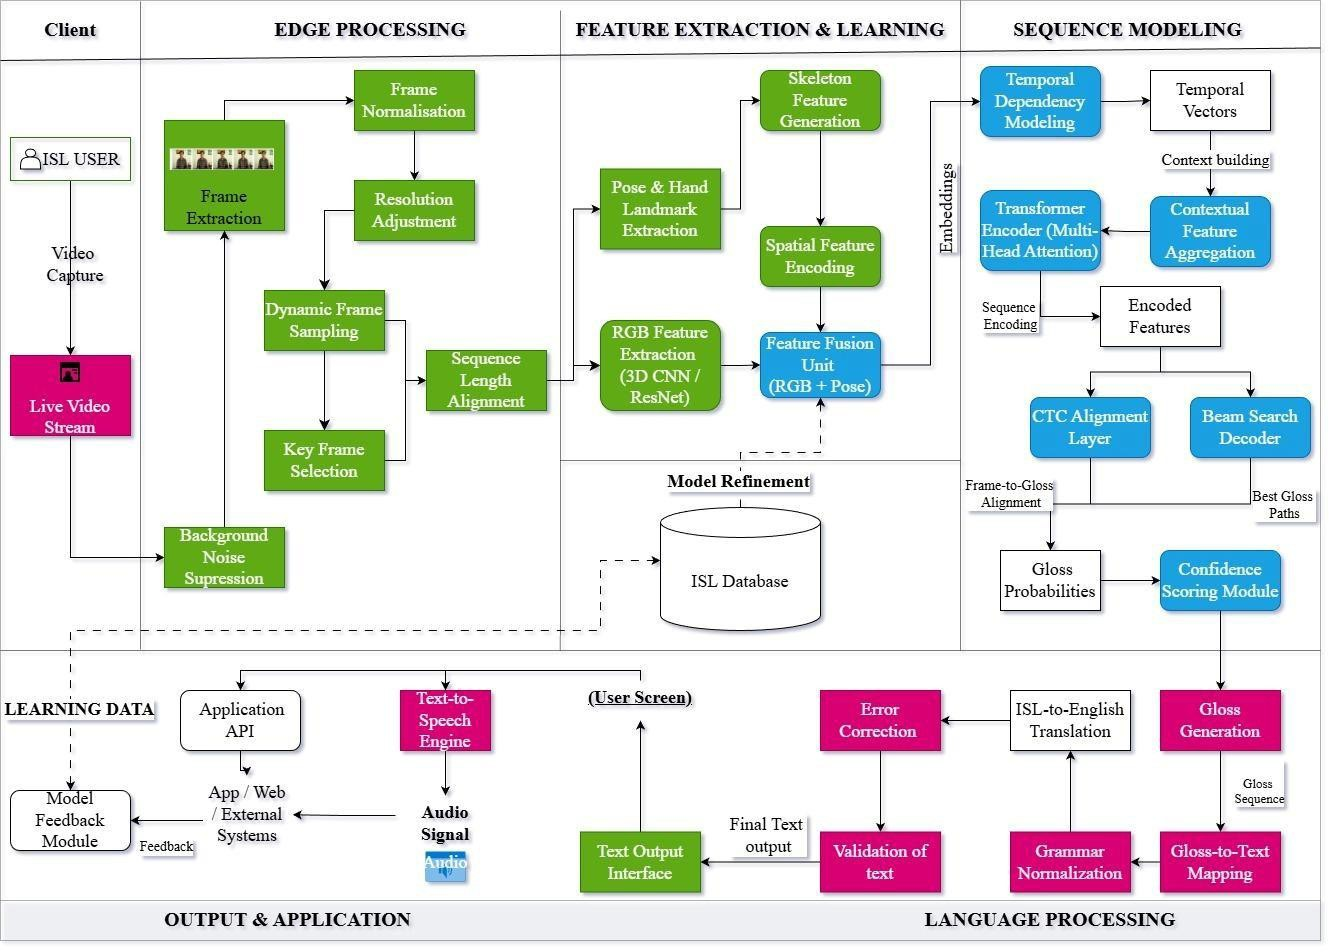
\includegraphics[width=\textwidth]{text/figures/docx_image1.jpeg}
\caption{Architecture diagram of proposed model.}
\label{fig:arch-proposed}
\end{figure}

\subsection{Block Diagram}
\subsubsection{Video Input Acquisition and Preprocessing}
The system takes an RGB video of ISL gestures as input. Since raw video cannot be directly used, preprocessing is performed. The video is first converted into frames using uniform sampling to preserve temporal information. Each frame is resized and normalized to ensure consistent input size and stable training. Additionally, all sequences are standardized to a fixed length using padding or truncation, enabling efficient batch processing.

\subsubsection{Spatial Feature Extraction Using EfficientNet}
EfficientNet is used to extract spatial features from each frame, such as hand shape, orientation, and appearance. The model is pretrained and adapted through transfer learning, generating compact feature vectors with high representation quality and computational efficiency.

\subsubsection{Temporal Feature Extraction Using CNN--RNN}
To capture motion information, a CNN--RNN architecture is used. CNN extracts frame-level features, and RNN processes them sequentially to learn temporal dependencies, including gesture movement, direction, and transitions over time.

\subsubsection{Multi-Feature Attention Mechanism}
The attention mechanism assigns weights to spatial and temporal features based on their importance. It focuses on relevant frames and suppresses less useful information, improving recognition accuracy and robustness to noise.

\subsubsection{Feature Fusion}
Spatial and temporal features are combined to create a unified representation. This fusion captures both visual appearance and motion dynamics of gestures, making the model more effective in recognizing complex signs.

\subsubsection{Sequence Modeling Using Transformer}
The fused features are passed to a Transformer encoder \cite{zhou2024transformer}, which models long-range dependencies using self-attention and captures relationships between frames efficiently.

\subsubsection{Temporal Alignment Using CTC}
CTC is used to align predicted outputs with input sequences without requiring exact frame-level labeling. This makes the system flexible and suitable for sequence-based gesture recognition.

\subsubsection{Decoding Using Beam Search}
Beam search is applied during prediction to select the most probable output sequence by evaluating multiple candidate sequences, improving overall accuracy compared to simple greedy decoding.

\subsubsection{Language Processing and Grammar Refinement}
The predicted gesture sequence is converted into text using mapping techniques. Grammar refinement is applied to correct sentence structure and improve readability.

\subsubsection{Output Generation and Text-to-Speech Conversion}
The final output is displayed as text and also converted into speech using a text-to-speech system. This enables effective communication between sign language users and non-signers.
